\section{Distribution of Floating-Point Roundoff Errors}\label{sec:errordist}

We briefly described in the GPS example of \cref{sec:overview} how our tool \Tool computes \emph{probabilistic} roundoff errors by conditioning the optimization of symbolic affine form (presented in the next section) on the output of the computation landing in a confidence interval.  The purpose of this section is to provide the necessary probabilistic tools to compute these intervals. Specifically, we will show how the probabilistic model of \cref{eq:probabilistic} can be used to compute (or at least bound) the output distribution of a probabilistic computation in finite-precision. In other words, this section provides the foundations of \emph{probabilistic range analysis}.

Our first task is to specify the distribution $dist$ of the random variable $\delta$ in the probabilistic model given by \cref{eq:probabilistic}.  Following \cite{dahlqvist2019probabilistic},  we use the fact that $dist$ can be computed explicitly from first principles and expressed in closed form (\cref{eq:LPerrorDensity}).  However,  this expression can only be computed in practice at very low precision. We then show that roundoff error distributions in high precision (say, single-precision and higher) can be approximated by another closed-form expression \cref{eq:HPerrorDensity} with an error that can be explicitly bounded, allowing us to remain sound.  Moreover, the quality of this approximation increases with the working (\ie benchmark) precision.  In the case where all mantissas are equiprobable,  it can be shown that as the working precision increases,  the roundoff error distribution always converges to a unique distribution given by \cref{eq:typicalpdf}, which we call the \emph{typical distribution}.  
For this class of input distributions, the distribution of errors is therefore asymptotically independent of the way the inputs are distributed.  More generally, we show that the covariance between the roundoff errors of \cref{eq:HPerrorDensity} and their generating input distribution is extremely small, that is to say the two processes are almost completely uncorrelated. This will have an important practical application when evaluating our probabilistic model of IEEE 754 arithmetic presented in \cref{subsec:model}. All proofs can be found in the Appendix.

\subsection{Derivation of the Distribution of Rounding Errors}\label{subsec:LPerror_dist}

Let us return to the probabilistic model of IEEE 754 arithmetic given by \cref{eq:probabilistic} where $\iop$ is the infinite-precision arithmetic operation and $\mop$ is its finite-precision implementation:
\[
z_1\mop z_2=(z_1\iop z_2)(1+\delta) \qquad\delta\sim dist.
\]
Let us also assume that $z_1,z_2$ are random variables with known distributions.  Then $z_1\iop z_2$ is also a random variable which can (in principle) be computed. Since the IEEE 754 standard states that $z_1\mop z_2$ should be given by rounding the infinite precision operation $z_1\iop z_2$, it is a completely natural consequence of the standard to require that $\delta$ should simply be given by 
\[
\delta = \erel(z_1\iop z_2).
\]
Thus $dist$ should simply be the distribution of the random variable $\erel(z_1\iop z_2)$. 
More generally, if $X$ is a random variable with know distribution, we will show how to compute the distribution $dist$ of the random variable
\[
\erel(X)=\frac{X-\round(X)}{X}.
\]
We choose to express the distribution $dist$ of relative errors \emph{in multiples of the unit roundoff $\uro$}. This choice is arbitrary, but it allows us to work with a distribution on the conceptually and numerically convenient interval $\left[-1,1\right]$, since the absolute value of the relative error is strictly bounded by $\uro$ (see \cref{subsec:fparith}), rather than the interval $\left[-\uro,\uro\right]$. 

To compute the density function of $dist$, we proceed as described in \cref{subsec:prob} by first computing the CDF $c(t)$ and then taking its derivative.  Recall first from \cref{subsec:fparith} that $\erel(x)=1$ if $x\in \fintvl[0]\setminus\{0\}$,  $\erel(x)=\infty$ if $x\in \fintvl[-\infty]$,  $\erel(x)=-\infty$ if $x\in \fintvl[\infty]$, and $-u \leq \erel(x)\leq u$ elsewhere.  Thus:
\begin{align*}
& \Pro{\erel(X)=-\infty}=\Pro{X\in\fintvl[\infty]} 
& \Pro{\erel(X)=1}=\Pro{X\in\fintvl[0]} \\
& \Pro{\erel(X)=\infty}=\Pro{X\in\fintvl[-\infty]}
\end{align*}
In other words, the probability measure corresponding to $\erel$ has three discrete components at $\{-\infty\}, \{1\}$,  and $\{\infty\}$, which cannot be accounted for by a PDF (see \cref{subsec:prob}).  It follows that the probability measure $dist$ is given by
\begin{align}
dist_c + \Pro{X\ssvin\fintvl[0]}\delta_1 + \Pro{X\ssvin\fintvl[-\infty]}\delta_{\infty}\ \hspace{-3pt}+ \Pro{X\ssvin\fintvl[\infty]}\delta_{-\infty}\label{eq:densitydecomp}
\end{align}
where $dist_c$ is a continuous measure that is not quite a probability measure since its total mass is $1-\Pro{X\in\fintvl[0]}-\Pro{X\ssvin\fintvl[-\infty]} - \Pro{X\ssvin\fintvl[\infty]}$. 
In general, $dist_c$ integrates to 1 in machine precision since $\Pro{X\in\fintvl[0]}$ is of the order of the smallest positive floating-point representable number, and the PDF of $X$ rounds to 0 way before it reaches the smallest/largest floating-point representable number. For example, Python's \texttt{scipy} implementation of the PDF of the standard Gaussian rounds to 0 from $x=39$.  However in order to be sound, we must in general include these three discrete components in our computations. The density $dist_c$ can be computed explicitly and is given by the following result whose proof can essentially be found in \cite{dahlqvist2019probabilistic}.

\begin{theorem}\label{thm:LP_errorDensity}
Let $X$ be a real random variable with PDF $f$. The continuous part $dist_c$ of the distribution of $\erel(X)$ has a PDF given by
\begin{align}
d(t)=\sum_{z\in\F\setminus\{-\infty,0,\infty\}}\one_{\fintvl[z]}\left(\frac{z}{1-t\uro}\right) f\left(\frac{z}{1-t\uro}\right) \frac{\uro\absv{z}}{(1-t\uro)^2},\label{eq:LPerrorDensity}
\end{align}
where $\one_{A}(x)$ is the indicator function which returns 1 if $x\in A$ and 0 otherwise. 
\end{theorem}

\begin{figure}[tb]
\centering
\begin{tabular}{l l l}
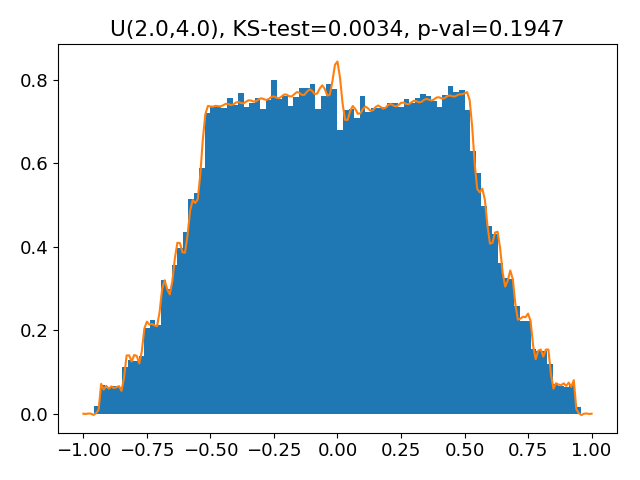
\includegraphics[scale=0.25]{pics/Error_U_2_4_4_3.png}
&
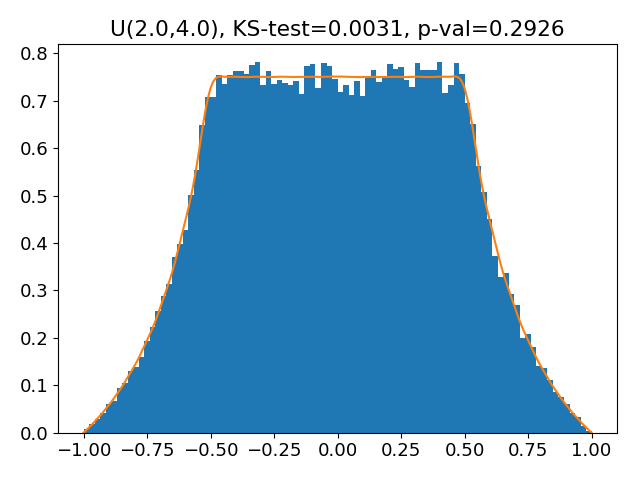
\includegraphics[scale=0.25]{pics/Error_U_2_4_11_5.png}
&
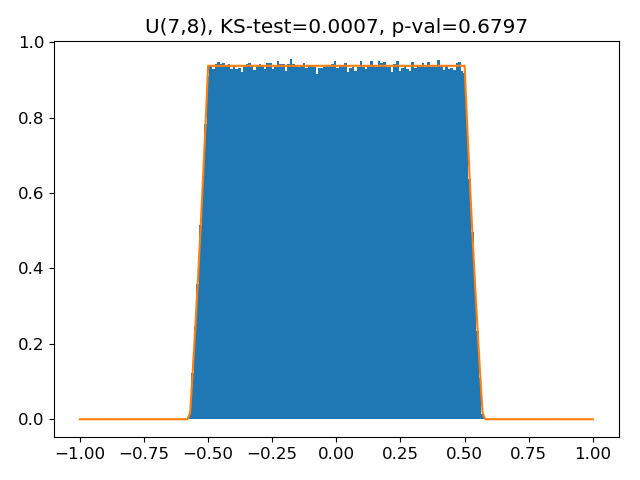
\includegraphics[scale=0.25]{pics/Error_U_7_8.png}
\\
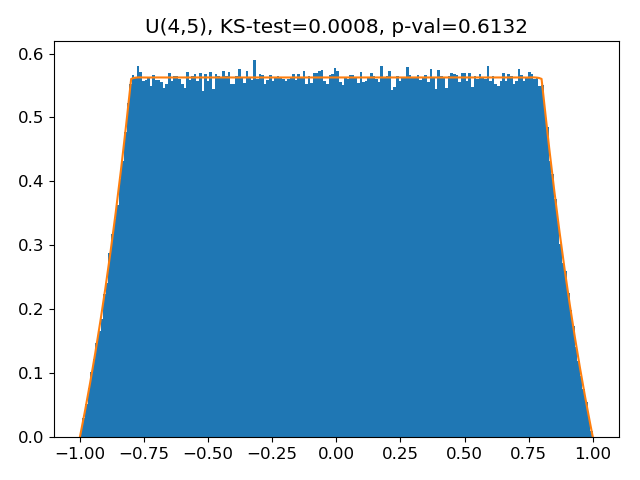
\includegraphics[scale=0.25]{pics/Error_U_4_5.png}
&
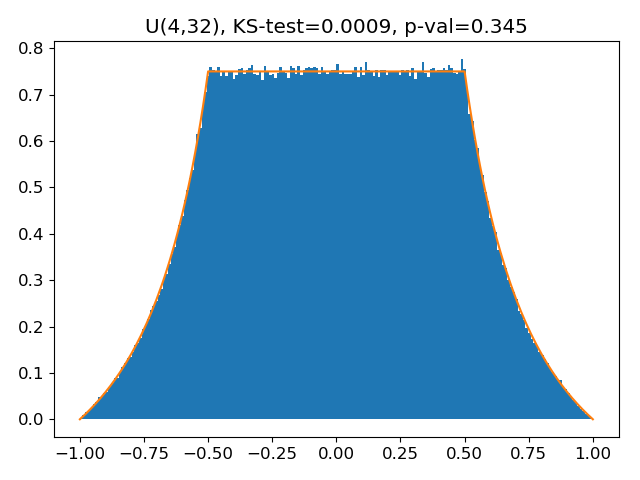
\includegraphics[scale=0.25]{pics/Error_U_4_32.png}
&
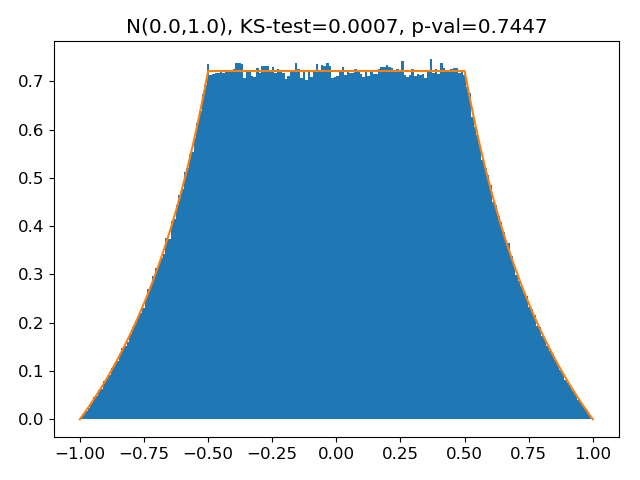
\includegraphics[scale=0.25]{pics/Error_N_0_1.png}
\end{tabular}
\caption{Error distribution versus the corresponding empirical error distributions, clockwise from top-left: (i) \cref{eq:LPerrorDensity} for $\uniform{2}{4}$ 3 bit exponent,  4 bit significand,  (ii) \cref{eq:LPerrorDensity} for $\uniform{2}{4}$ in half-precision,  (iii) \cref{eq:HPerrorDensity} for $\uniform{7}{8}$ in single-precision, (iv) \cref{eq:HPerrorDensity} for $\uniform{4}{5}$ in single-precision, (v) \cref{eq:HPerrorDensity} for $\uniform{4}{32}$ in single-precision, (vi) \cref{eq:HPerrorDensity} for $\normal{0}{1}$ in single-precision.}
\label{fig:error_dist}
\end{figure}

\cref{fig:error_dist} (i) and (ii) shows an implementation of \cref{eq:LPerrorDensity} applied to the distribution $\uniform{2}{4}$, first in very low precision (3 bit exponent, 4 bit significand) and then in half-precision. The theoretical density is plotted alongside a histogram of the relative error incurred when rounding 100,000  samples to low precision (computed in double-precision).  The reported statistic is the K-S (Kolmogorov-Smirnov) test which measures the likelihood that a collection of samples were drawn from a given distribution. This test reports that we cannot reject the hypothesis that the samples are drawn from the corresponding density. Note how in low precision the term in $\frac{1}{(1-t\uro)^2}$ induces a visible asymmetry on the central section of the distribution. This effect is much less pronounced in half-precision.


For low precisions, say up to half-precision, it is computationally feasible to explicitly go through all floating-point numbers and compute the density of the roundoff error distribution $dist$ directly from \cref{eq:LPerrorDensity}. However, this rapidly becomes prohibitively computationally expensive for higher precisions (since the number of floating-point representable numbers grows exponentially).

\subsection{High-Precision Case} \label{subsec:HPerror_dist}

As the working precision increases, a regime changes occurs: on the one hand it becomes practically impossible to enumerate all floating-point representable numbers as done in \cref{eq:LPerrorDensity}, but on the other hand sufficiently well-behaved density functions are numerically close to being constant at the scale of an interval between two floating-point representable numbers. We exploit this smoothness to overcome the combinatorial limit imposed by \cref{eq:LPerrorDensity}.

\begin{theorem}\label{thm:HP_errorDensity}
Let $X$ be a real random variable with PDF $f$. The continuous part $dist_c$ of the distribution of $\erel(X)$ has a PDF given by
$d_c(t) = d_{hp}(t) + R(t)$
where $d_{hp}(t)$ is the function on $[-1,1]$ defined by
\begin{align}
d_{hp}(t)=
\begin{cases}
 \frac{1}{1-t\uro}\sum\limits_{s, e=\emin+1}^{\emax-1} \int_{(-1)^s2^e(1-\uro)}^{(-1)^s2^e(2-u)} \frac{\absv{x}}{2^{e+1}} f(x) ~dx & \absv{t}\leq \frac{1}{2}\\
\\
\frac{1}{1-t\uro}\sum\limits_{s, e=\emin+1}^{\emax-1} \int_{(-1)^s2^e(1-\uro)}^{(-1)^s2^e(\frac{1}{\absv{t}}-\uro)} \frac{\absv{x}}{2^{e+1}} f(x) ~dx  &\frac{1}{2}<\absv{t}\leq 1
\end{cases}\label{eq:HPerrorDensity}
\end{align}
and $R(t)\hspace{-1pt}$ is an error whose total contribution $\absv{R}\hspace{-2pt}\defeq \hspace{-3pt}\int_{-1}^{1}\hspace{-2pt}\absv{R(t)}\hspace{-1pt}dt$ can be bounded by
\begin{align*}
\absv{R}\leq  & ~\Pro{\round(X)=z(s,\emin, k)} +  \Pro{\round(X)=z(s,\emax, k)}  + \\
&\frac{3}{4} \left(\sum_{s, \emin<e<\emax} \absv{f'(\xi_{e,s})\xi_{e,s} + f(\xi_{e,s})}\frac{2^{2e}}{2^{p}}\right)
\end{align*}
where for each exponent $e$ and sign $s$, $\xi_{e,s}$ is a point in $[z(s,e,0), z(s,e,2^{p}-1)]$ if $s=0$ and in $[z(s,e,2^{p}-1), z(s,e,0)]$ if $s=1$.
\end{theorem}

Note how \cref{eq:HPerrorDensity} reduces the sum over \emph{all} floating-point representable numbers in \cref{eq:LPerrorDensity} to a sum over \emph{the exponents} by exploiting the regularity of $f$. This can often be reduced further since one only needs to consider the exponent on the support of $f$. Note also that since $f$ is a PDF, it usually decreases very quickly away from 0, and its derivative decreases even quicker (or vanishes altogether for uniform distributions) and $\absv{R}$ thus tends to be very small.  This is the case for all benchmarks in \cref{sec:evaluation}.  As an example, in single-precision for $X\sim\normal{0}{1}$ we get $\absv{R}<\mathtt{3.2e-7}$, for $X\sim\uniform{-2}{2}$ we get  $\absv{R}<\mathtt{1.2e-7}$; in both cases very close to the smallest floating-point representable increment to 1. Moreover, $\absv{R}\to 0$ as the precision $p\to\infty$.

\cref{eq:HPerrorDensity} is easy to implement, and we present some results in \cref{fig:error_dist} where we have chosen as input: (i) a distribution $\uniform{7}{8}$ where large significands are more likely, (ii) a distribution $\uniform{4}{5}$ where small significands are more likely, (iii) a distribution $\uniform{4}{32}$ where all significands are equally likely, and (iv) a distribution $\normal{0}{1}$ with infinite support. The graphs show the density function given by \cref{eq:HPerrorDensity} in single-precision versus a histogram of the relative error incurred when rounding 1,000,000  samples to single-precision (computed in double-precision).  The K-S test reports that we cannot reject the hypothesis that the samples are drawn from the corresponding distributions.

\subsection{Typical Distribution}\label{subsec:typical}
The distributions depicted in graphs (ii), (v) and (vi) of \cref{fig:error_dist} are extremely similar, despite being computed from very different input distributions. What they have in common is that their input distributions have the property that that all significands in their supports are equally likely.  In fact, we show that under this 
\begin{wrapfigure}{r}{0.48\textwidth}
\vspace{-7mm}
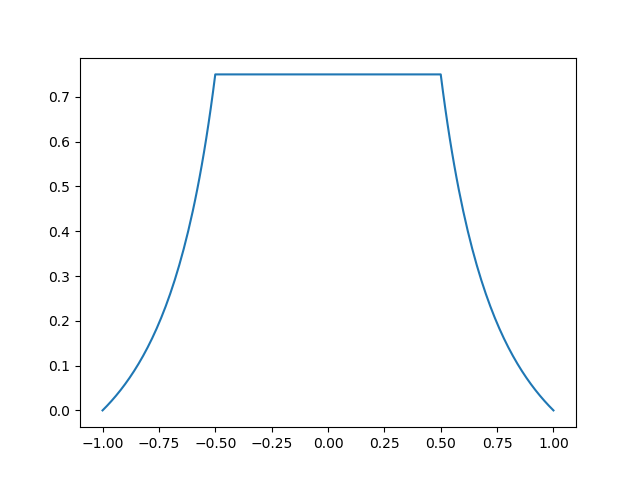
\includegraphics[width=0.52\textwidth]{pics/typical_dist.png}
\captionof{figure}{Typical distribution.}
\label{fig:typical}
\end{wrapfigure}
assumption,  the distribution of roundoff errors given by \cref{eq:LPerrorDensity} converges to a unique density 
as the precision increases, irrespective of the input distribution! 
Since all significands are in practice often equiprobable (it is the case for a third of the benchmarks presented in \cref{sec:evaluation}), this density is of great practical importance.  If one had to choose `the' canonical distribution for roundoff errors, we claim that the density given below should be this distribution, and we therefore call it the \emph{typical distribution}; we depict it in \cref{fig:typical} and formalize it with the following theorem, which makes precise ideas from \cite{dahlqvist2019probabilistic}.

\begin{theorem}\label{thm:typical_dist}
If $X$ is a random variable such that $\Pro{\round(X) = z(s,e,k_0)}=\frac{1}{2^p}$ for any significand $k_0$, then
\begin{align}
d_{typ}(t)\defeq \lim_{p\to\infty} d(t) = \begin{cases}
\frac{3}{4}&\absv{t}\leq\frac{1}{2}
\\
\frac{1}{2}\left(\frac{1}{t}-1\right)+\frac{1}{4}\left(\frac{1}{t}-1\right)^2 & \absv{t}>\frac{1}{2}
\end{cases}\label{eq:typicalpdf}
\end{align} 
where $d(t)$ is the exact density given by \cref{eq:LPerrorDensity}.
\end{theorem}

\subsection{Covariance Structure}\label{subsec:covar}

The result above can be interpreted as saying that if $X$ is such that all mantissas are equiprobable, then $X$ and $\erel(X)$ are asymptotically independent (as $p\to\infty$).  Much more generally,  we now show that if a random variable $X$ has a sufficiently regular PDF, it is close to being uncorrelated from $\erel(X)$. Formally, we prove that the covariance 
\begin{align}
\cov(X,\erel(X)) = \Exp{X.\erel(X)}-\Exp{X}\Exp{\erel(X)}
\label{eq:covdef}
\end{align}
is small, specifically of the order of $\uro$. Note that the expectation in the first summand above is taken \wrt the joint distribution of $X$ and $\erel(X)$.

The main technical obstacles to proving that the expression above is small are that $\Exp{\erel(X)}$ turns out to be difficult to compute (we only manage to bound it) and that the joint distribution
$\Pro{X\in A \wedge \erel(X) \in B}$
does not have a PDF since it is not continuous \wrt the Lebesgue measure on $\R^2$. Indeed, it is supported by the graph of the function $\erel$ which has a Lebesgue measure of 0. This does not mean that it is impossible to compute the expectation
\begin{align}
\Exp{X.\erel(X)} = \int_{\R^2} x\uro t ~d\mathbb{P}\label{eq:expdef}
\end{align}
but it is necessary to use some more advanced probability theory.  We will make the simplifying assumption that the density of $X$ is constant at the level of each interval $\fintvl$ in order to keep the proof manageable.  In practice this is an extremely good approximation. Without this assumption, we would need to add an error term similar to that of \cref{thm:HP_errorDensity} to the expression below. This is not conceptually difficult, but is is rather messy, and it would distract from the main aim of the following theorem which is to bound $\Exp{\erel(X)}$, compute $\Exp{X.\erel(X)}$, and show that the covariance between $X$ and $\erel(X)$ is typically of the order of $\uro$.
\begin{theorem}\label{thm:covar}
If the density of $X$ is piecewise constant on intervals $\fintvl$,  then
\[
\left(L -  \Exp{X}K\frac{\uro}{6}\right) \leq \cov(X,\erel(X))\leq \left(L -  \Exp{X}K\frac{4\uro}{3}\right)
\]
where $L=\sum\limits_{s,e} f((-1)^s2^e)(-1)^s2^{2e}\frac{3\uro^2}{2}$ and $K=\hspace{-12pt} \sum\limits_{s,e=\emin+1}^{\emax-1}\int_{(-1)^s2^e(1-\uro)}^{(-1)^s2^e(2-u)} \frac{\absv{x}}{2^{e+1}} f(x) ~dx$
\end{theorem} 
If the distribution of $X$ is centered (i.e., $\Exp{X}=0$) then $L$ is the exact value of the covariance, and it is worth noting that $L$ is fundamentally an artefact of the floating-point representation and is due to the fact that the intervals $\fintvl[2^e]$ are not symmetric. More generally, for $\Exp{X}$ of the order of, say, 2, the covariance will be small (of the order of $\uro$) as $K\leq 1$ (since $\absv{x}\leq 2^{e+1}$ in each summand).  For very large values of $\Exp{X}$ it is worth noting that there is a high chance that $L$ is also be very large, partially canceling $\Exp{X}$. An illustration of this is given by the \textit{doppler} benchmark examined in \cref{sec:evaluation}, an outlier as it has an input variable with range $\left[20,~20000\right]$. Nevertheless,  even for this benchmark the bounds of \cref{thm:covar} still give a small covariance of the order of $0.001$.

\subsection{Error Terms and P-Boxes}\label{subsec:errorpbox}

In low-precision we can use the exact formula \cref{eq:LPerrorDensity} to compute the error distribution. However, in high-precision,  approximations (typically extremely good) like \cref{eq:HPerrorDensity,eq:typicalpdf} must be used. In order to remain sound in the implementation of our model (see \cref{sec:model}) we must account for the error made by this approximation. We have not got the space to discuss the error made by \cref{eq:typicalpdf}, but taking the term $\absv{R}$ of \cref{thm:HP_errorDensity} as an illustration, we can use the notion of p-box described in \cref{subsec:prob} to create an object which soundly approximates the error distribution. We proceed as follows: since $\absv{R}$ bounds the total error accumulated over all $t\in[-1,1]$, we can soundly bound the CDF $c(t)$ of the error distribution given by \cref{eq:HPerrorDensity} by using the p-box
\[
c^-(t)=\max(0,c(t)-\absv{R})\qquad\text{and} \qquad c^+(t)=\min(1,c(t)+\absv{R})
\]
This p-box is used as the (independent) roundoff error term for the probabilistic model of IEEE arithmetic given by \cref{eq:model}, which we describe in \cref{sec:model}.

